\chapter{Voltage peak transducer}
\section{Theory and related work} \label{sec:literature_voltage_peak_transducer}
The design chosen for this voltage peak transducer utilized a resistor divider network as well as a full wave precision rectifier. A resistor divider network is a series connection of two resistors and is used to decrease the magnitude of an input voltage to an acceptable level so that it can be measured. An important element in the design of this circuit is to minimise any current flow in the resistors, thus large resistor values must be chosen. A precision rectifier is an operational amplifier circuit configuration that allows a rectifier circuit to behave like an ideal diode and rectifier, an advantage of this circuit is that it allows the rectification of voltages smaller than the forward voltage of the diode \cite{PrecisionRectifier}.

\section{Design} \label{sec:design_voltage_peak_transducer}
The first step in this design was to design a circuit that would step the fairly large \SI{24}{VAC} input down to an analogue voltage usable by the operational amplifier circuitry, for simplicity a simple voltage divider network was chosen. It was found that the largest differential mode input to the TLC2272 was  $V_{DD}=\SI{5}{V}$ and the absolute minimum input was found as $V_{EE}-\SI{0.3}{V}=\SI{-0.3}{V}$ \cite{TLC2272:2016}. It was also found that each TLC2272 chip required roughly \SI{2.4}{\milli A} at room temperature given a supply voltage $V_{DD}=\SI{5}{V}$ \cite{TLC2272:2016}. Referring to Figure \ref{fig:system_diagram} we can see that this design required three of these chips, which translated to four operational amplifiers, and thus it was decided that for the voltage transducer a single supply would be used as to not exceed the limitations of the negative voltage supply rail specified in the first report. A 1N4007 diode was placed in series with the voltage divider to rectify this input as to not exceed the maximum negative differential mode input of \SI{-0.3}{V}.\vspace{4mm} \newline An absolute maximum input voltage of \SI{24}{VAC} was chosen and the forward voltage of the diode had to be compensated for, this was found to be 0.7V after choosing a maximum current of 0.4mA through the voltage divider resistors \cite{1N4007:2014}. Given this information the input to the resistor divider network was found to be $V_{in}=\SI{23.5}{VAC}$ and with the specified range of the Arduino being $4095$ bits it was calculated that for this maximum input voltage the resolution of the ADC would be $\SI{8.1175}{\milli V}$ per bit. The maximum current specification was used to calculate a minimum value of $\SI{10}{\kilo \Omega}$ for $R_{2}$. The value of $R_{1}$ was found by using Equation \ref{eq:voltagedivider} and rearranging the terms and substituting for the values. It was found that $R_{1}=\SI{56.6}{\kilo \Omega}$, hence a standard resistor value of $\SI{56}{\kilo \Omega}$ was chosen.
\begin{align}
   V_{DD}=\frac{R_2}{R_1+R_2}V_{in}
   \label{eq:voltagedivider}
\end{align}
The peak detection circuit chosen for this design was a simple full wave precision rectifier as can be seen in Figure \ref{fig:voltagepeakdetector.pdf} \cite{PrecisionRectifierFullwave}. To minimise any power losses in the operational amplifier, a resistor $R_3=\SI{10}{\kilo \Omega}$ was placed at its positive input pin to prevent an excess amount of current from flowing into the operational amplifier. Another resistor $R_4=\SI{10}{\kilo \Omega}$ was also placed between the non inverting input of the amplifier and the output as to ensure a minimum current flowing through to the output of the transducer during the negative half cycle of the input wave \cite{PrecisionRectifierFullwave}. 
If negative voltages are applied at the input of the precision rectifier the operational amplifier runs open loop, since the diode is reverse biased, which causes the operational amplifier to saturate. It takes time for the operational amplifier to move out of saturation, and this greatly decreases the frequency response of the circuit, thus further motivating the choice of rectifying the input voltage and supplying the operational amplifier with a single supply configuration \cite{PrecisionRectifierSaturation}. It is worth noting that the resistor $R_4$ is redundant due to the fact that the input has been rectified. \vspace{4mm} \newline
The final part of the peak detection circuit requires a capacitor and resistor with an adequate RC constant as to maintain the desired peak voltage to be measured by the Arduino. A ripple voltage of no more than $\SI{5}{\milli V}$ was chosen for this design and the required capacitor could then be found by using Equation \ref{eq:ripplevoltage}. With a maximum input voltage $V_{m}=\SI{5}{V}$, a frequency of \SI{50}{Hz} and the internal resistance of the Arduino's pins specified as $R=\SI{1}{M\Omega}$ it was found that the desired capacitor value had to be equal to $C=\SI{20}{\micro F}$ \cite{Neaman:2018}.\newline
\begin{align}
  V_{r} = \frac{V_{m}}{fRC} 
   \label{eq:ripplevoltage}
\end{align}
To ensure that the transducer met the design requirement of responding to a $\SI{1}{V}$ change, which corresponds to an output voltage change of $\SI{151.15}{\milli \volt}$, within 1 second, Equation \ref{eq:capacitordischarge} had to be used \cite{CapacitorDischarge}. Here $V_{s}=\SI{3.4284}{\volt}$, which corresponds to an input of \SI{16}{VAC}, and $V_{c}=\SI{3.2769}{\milli \volt}$, which corresponds to a \SI{1}{V} decrease in input peak voltage. An appropriate smoothing capacitor could now be calculated, as the equivalent input resistance of the Arduino was equal to $R=\SI{1}{M \Omega}$ and with the voltage changes measured before, the capacitor value was found to be $C=\SI{22.12}{\micro F}$. Noise on the output of this transducer had to be minimized thus two low ESR rated \SI{10}{\micro F} capacitors were placed in parallel to make an equivalent capacitance of \SI{20}{\micro F}. Decoupling capacitors were also placed at the positive voltage supply input to the TLC2272 to minimize any effects of noise from the power supply on the output of the transducer.
\begin{align}
  V_{c} = V_{s}e^{\frac{-t}{RC}} \nonumber \\
  C = \frac{t}{(\ln(\frac{V_{s}}{V_{c}}))R} \label{eq:capacitordischarge}
\end{align}

\begin{figure}[h!]
    \centering
    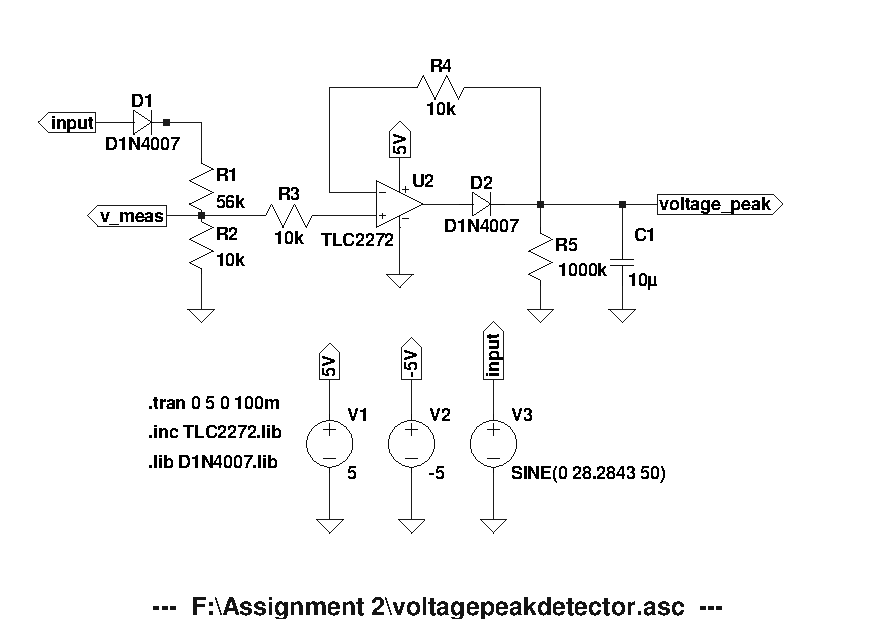
\includegraphics[width = 0.65\linewidth]{Figures/voltagepeakdetector.pdf}
        \caption{Voltage Peak Transducer Circuit Diagram}
    \label{fig:voltagepeakdetector.pdf}
\end{figure}


\section{Simulation} \label{sec:simulation_voltage_peak_transducer}
Firstly the designed voltage transducer was simulated given a nominal input voltage of $\SI{16}{VAC}$ and the plot of this output can be seen in Figure \ref{subfig:16VACinputripple}. From this graph it can be seen that the transducer perfectly follows the input wave at steady state. The voltage transducers response to a $\SI{1}{\volt}$ change in a $\SI{16}{VAC}$ input was simulated by using a piece wise linear voltage source to increase the input voltage by $\SI{1}{\volt}$, this output can be seen in Figure \ref{subfig:16VACinputchange}. From this graph we can see that the voltage transducer responded to the change in input within 1 second.

\begin{figure}[h!]
 \centering
     \begin{subfigure}[]{0.45\textwidth}
        \centering
         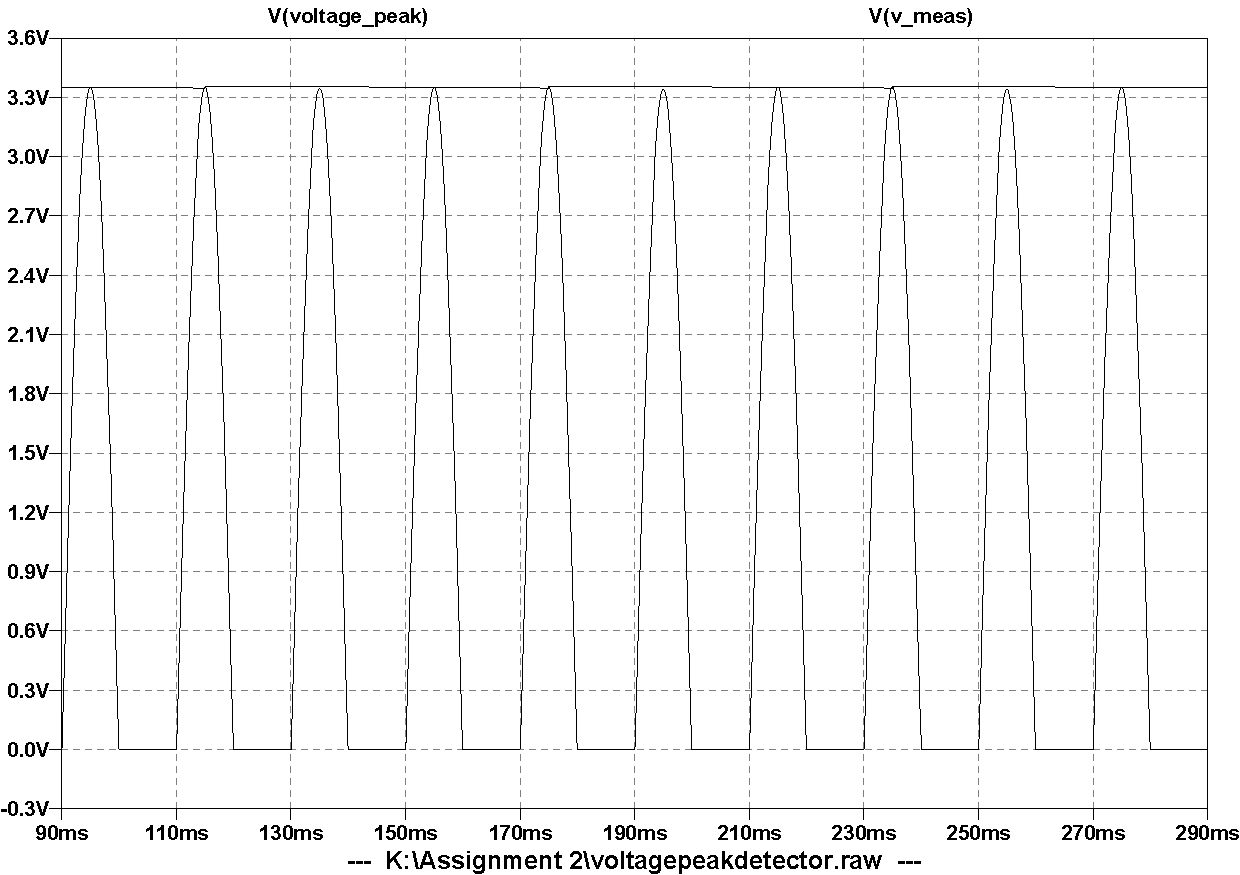
\includegraphics[width=1\linewidth]{./Figures/voltagepeakdetectoroutputsim.pdf}
		    \caption{Peak detection of scaled down \SI{16}{\volt AC} input.} \label{subfig:16VACinputripple}
     \end{subfigure}
      \begin{subfigure}[]{0.45\textwidth}
              \centering
  		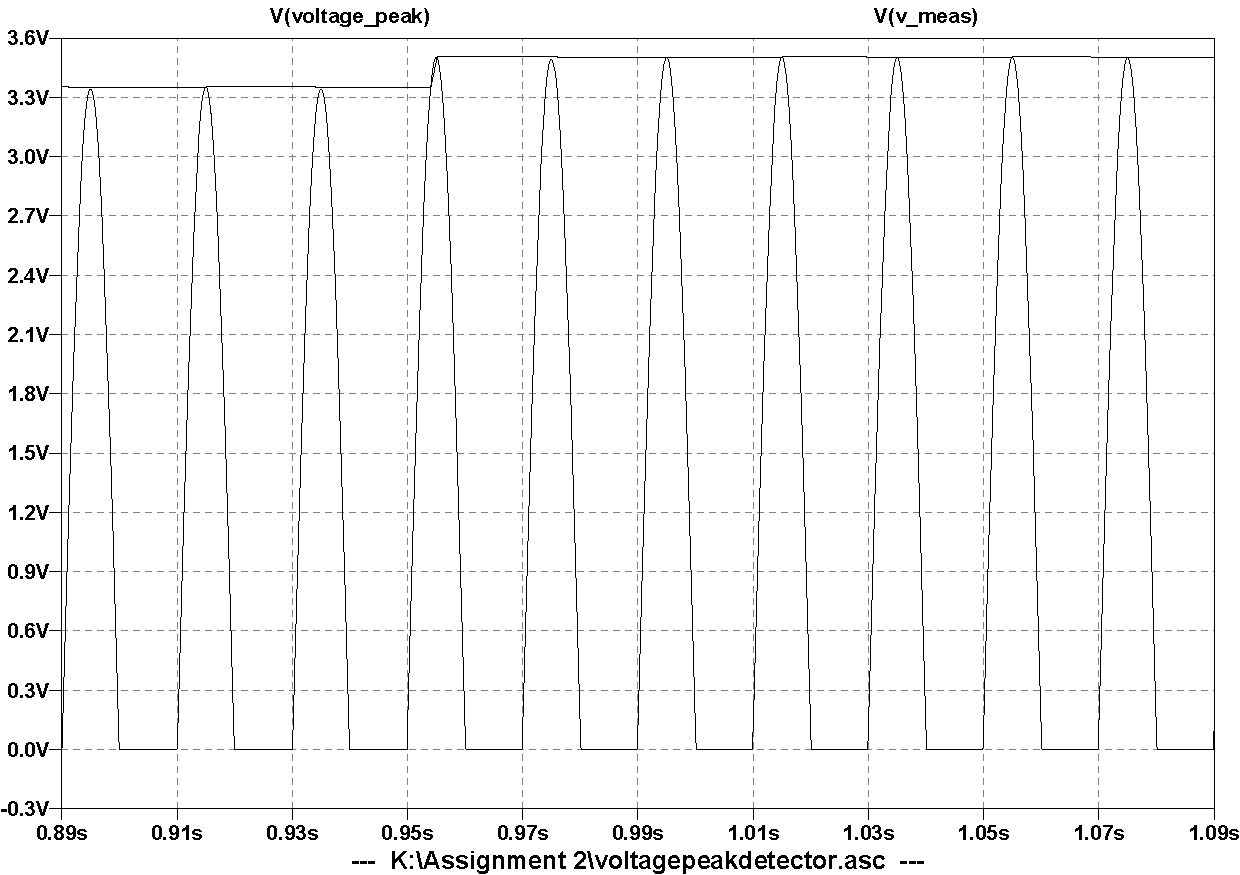
\includegraphics[width=1\linewidth]{./Figures/voltagepeakdetectoroutputchange.pdf}
		    \caption{Response given \SI{1}{\volt} change in \SI{16}{\volt AC} input.} \label{subfig:16VACinputchange}
     \end{subfigure}
   \caption[Simulated results for the voltage transducer]{Output voltage ripple and response for the voltage transducer. (a) depicts output voltage ripple, (b) depicts response to change in input. }
    \label{fig:voltage_simulation_results_box}
 \end{figure}

\section{Measurements} \label{sec:measurement_voltage_peak_transducer}
Unit tests were completed using a signal generator applied at the input of the voltage peak transducer to simulate various input voltages, these results can be seen in Table \ref{tab:voltagetransducerunittests}. All of these measurements were measured accurately and the applied input was deduced using Equation \ref{eq:pleaseworkthistimebru} with a maximum difference of only $\SI{83.12}{\milli \volt}$. Equation \ref{eq:voltagedelta} was then constructed to determine the effect of noise on the output. The transducer was also tested using the transformer as input under various load conditions with these results tabulated in Table \ref{tab:voltagetransducerrealtests}. Under all load conditions the deduced input differed from the actual input by no more than $\SI{118}{\milli \volt}$, confirming that the design met all requirements. The output of the voltage peak transducer, given an input from the transformer and a load of $\SI{1}{\kilo \Omega}$, can be seen in Figure \ref{subfig:voltagetransducermidrangereal}, with the quality of this signal shown in Figure \ref{subfig:16VACinputchangereal}. From this it was found that the transducer can accurately detect the peak of an input voltage with a maximum output noise below $\SI{10}{\milli \volt}$.
\begin{align}
  V_{meas} = (V_{load}-V_{\gamma})\frac{R_1}{R_1+R_2} \nonumber  \\
  V_{meas} = (V_{load}-0.7)0.14374 \label{eq:pleaseworkthistimebru} \\
  \delta v_{meas} = 0.14374\delta v_{load}\label{eq:voltagedelta}
\end{align}

\newcolumntype{C}[1]{>{\centering\arraybackslash}m{#1}}
\begin{table} [h!]
        \centering
        \footnotesize
        \caption{Voltage transducer intermediate unit test results.}
             \begin{tabular}{C{2cm} C{2cm} C{2cm} C{2cm} C{2cm} C{2cm}}
           Emulated level & Signal generator & Signal generator & Analogue output & Deduced input & Difference \\
           ($V_{peak}$)   & ($V_{peak}$)   & ($V_{peak}$)   & ($VDC$)         & ($V_{peak}$)  & ($mV_{peak}$) \\
           \hline
            16      & 2.034 & 2.196 & 2.208 & 16.081 & 83.12 \\
            21      & 2.736 & 2.915 & 2.916 & 21.009 & 8.67\\
            21.15   & 2.764 & 2.936  & 2.940 & 21.174 & 23.55 \\
            21.30   & 2.784 & 2.958 & 2.960 & 21.318 & 17.98 \\
            26      & 3.463 & 3.634 & 3.626 & 25.946 & 53.96\\
          \hline
        \end{tabular}
     \label{tab:voltagetransducerunittests}
\end{table}

\begin{table}
        \centering
        \footnotesize
        \caption{Voltage transducer integrated test results.}
         \begin{tabular}{C{1.9cm} C{1.2cm} C{1.2cm} | C{2.5cm} C{2.6cm} C{2.5cm} C{1.8cm}}
           Measurement & Load R & Load C  & Measured input & Analogue output & Deduced input & Difference\\
            & ($\Omega$) & ($\mu F$) & ($V_{peak}$) & ($VDC$) & ($V_{peak}$) & ($mV_{peak}$) \\
        \hline
            No load      & open & none & 30.38 & 4.270 & 30.406  & 26 \\
            Full load    & 100  & none & 29.12 & 4.140 & 29.224  & 104 \\
            Mid range    & 1k   & none & 30.08 & 4.240 & 30.198  & 118\\
          \hline
        \end{tabular}
     \label{tab:voltagetransducerrealtests}
\end{table}

\begin{figure}[h!]
 \centering
     \begin{subfigure}[]{0.45\textwidth}
        \centering
         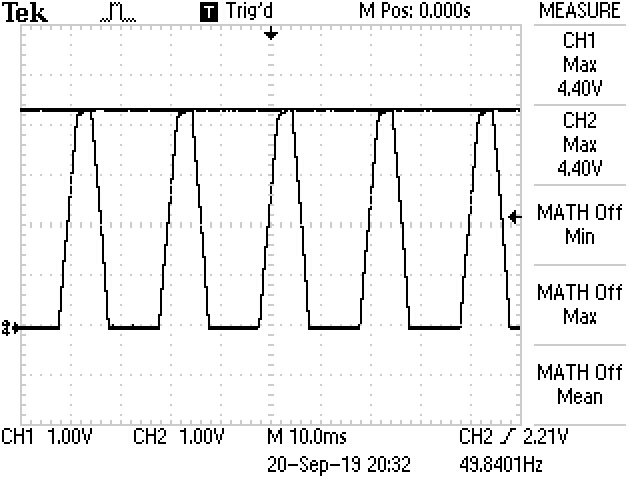
\includegraphics[width=1\linewidth]{./Figures/voltagetransducermidrange.JPG}
		    \caption{Mid range measurement result} \label{subfig:voltagetransducermidrangereal}
     \end{subfigure}
      \begin{subfigure}[]{0.45\textwidth}
              \centering
  		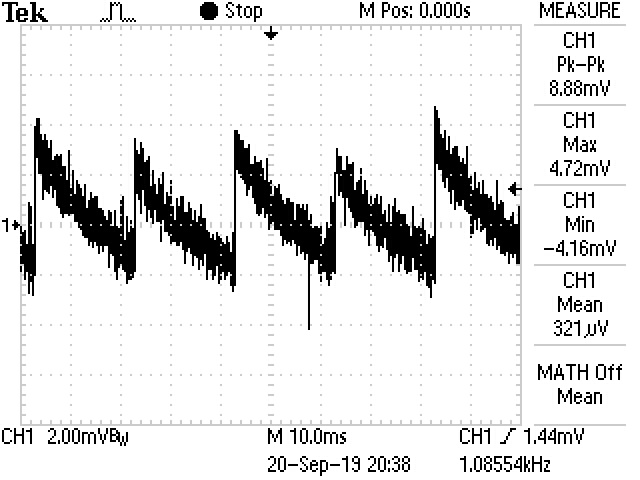
\includegraphics[width=1\linewidth]{./Figures/voltagetransducernoise.JPG}
		    \caption{Noise response} \label{subfig:16VACinputchangereal}
     \end{subfigure}
   \caption[Measured results for the voltage transducer]{Output voltage ripple and response for the voltage transducer. (a) depicts mid range output, (b) depicts noise response. }
    \label{fig:simulation_results_box}
 \end{figure}